\documentclass[12pt]{article}
\usepackage[utf8]{inputenc}
\usepackage{listings}
\usepackage{setspace}
\usepackage{graphicx}
\usepackage{hyperref}
\usepackage{amsmath}
\usepackage{booktabs}
\usepackage{csquotes}
\usepackage{cases}
\usepackage{titling}
\usepackage{blindtext}
\usepackage{float}
\usepackage{amssymb}
\usepackage{mathtools}
\usepackage{subcaption}
\usepackage{lipsum}
\usepackage[left=2.5cm,top=2.5cm,right=2.5cm,bottom=2.5cm]{geometry}
\setlength{\parindent}{0pt}

\doublespacing
\hypersetup{
    colorlinks=true,
    linkcolor=blue,
    filecolor=magenta,      
    urlcolor=cyan,
}

%\renewcommand{\familydefault}{\sfdefault}

\title{CTA200 Project}
\author{Feiyu Quan}
\date{May 2022}


\begin{document}

\maketitle

\section{Introduction}

The goal of this project is to get a hands-on experience and understanding of the output from TNG50, a large cosmological MHD simulation of galaxies. We use \texttt{Python} packages such as \texttt{h5py} and \texttt{numpy} to manipulate the data, and \texttt{matplotlib} for the visualization. The simulation data used in this project can be found at: \url{https://www.tng-project.org/api/TNG50-1/snapshots/99/subhalos/117258/}.


\section{Part 1}

We first convert the unit of coordinates of the stellar particles in the simulation box from ckpc/h to the physical kpc. Here the first \enquote{c} in \enquote{ckpc} refers to the comoving distance. To do this, we multiply the comoving distance by the Hubble factor $h = 0.6774$ (\url{https://arxiv.org/pdf/1902.05553.pdf}, section 2.1).

Now with the physical coordinates, we plot the surface density of the stellar masses in the x-y plane, by weighting a histogram of number of stellar particles with their masses and then dividing by the surface element ${\rm d}x {\rm d}y$. The plot is shown in Figure \ref{Fig1}.

\begin{figure}[ht]
    \centering
    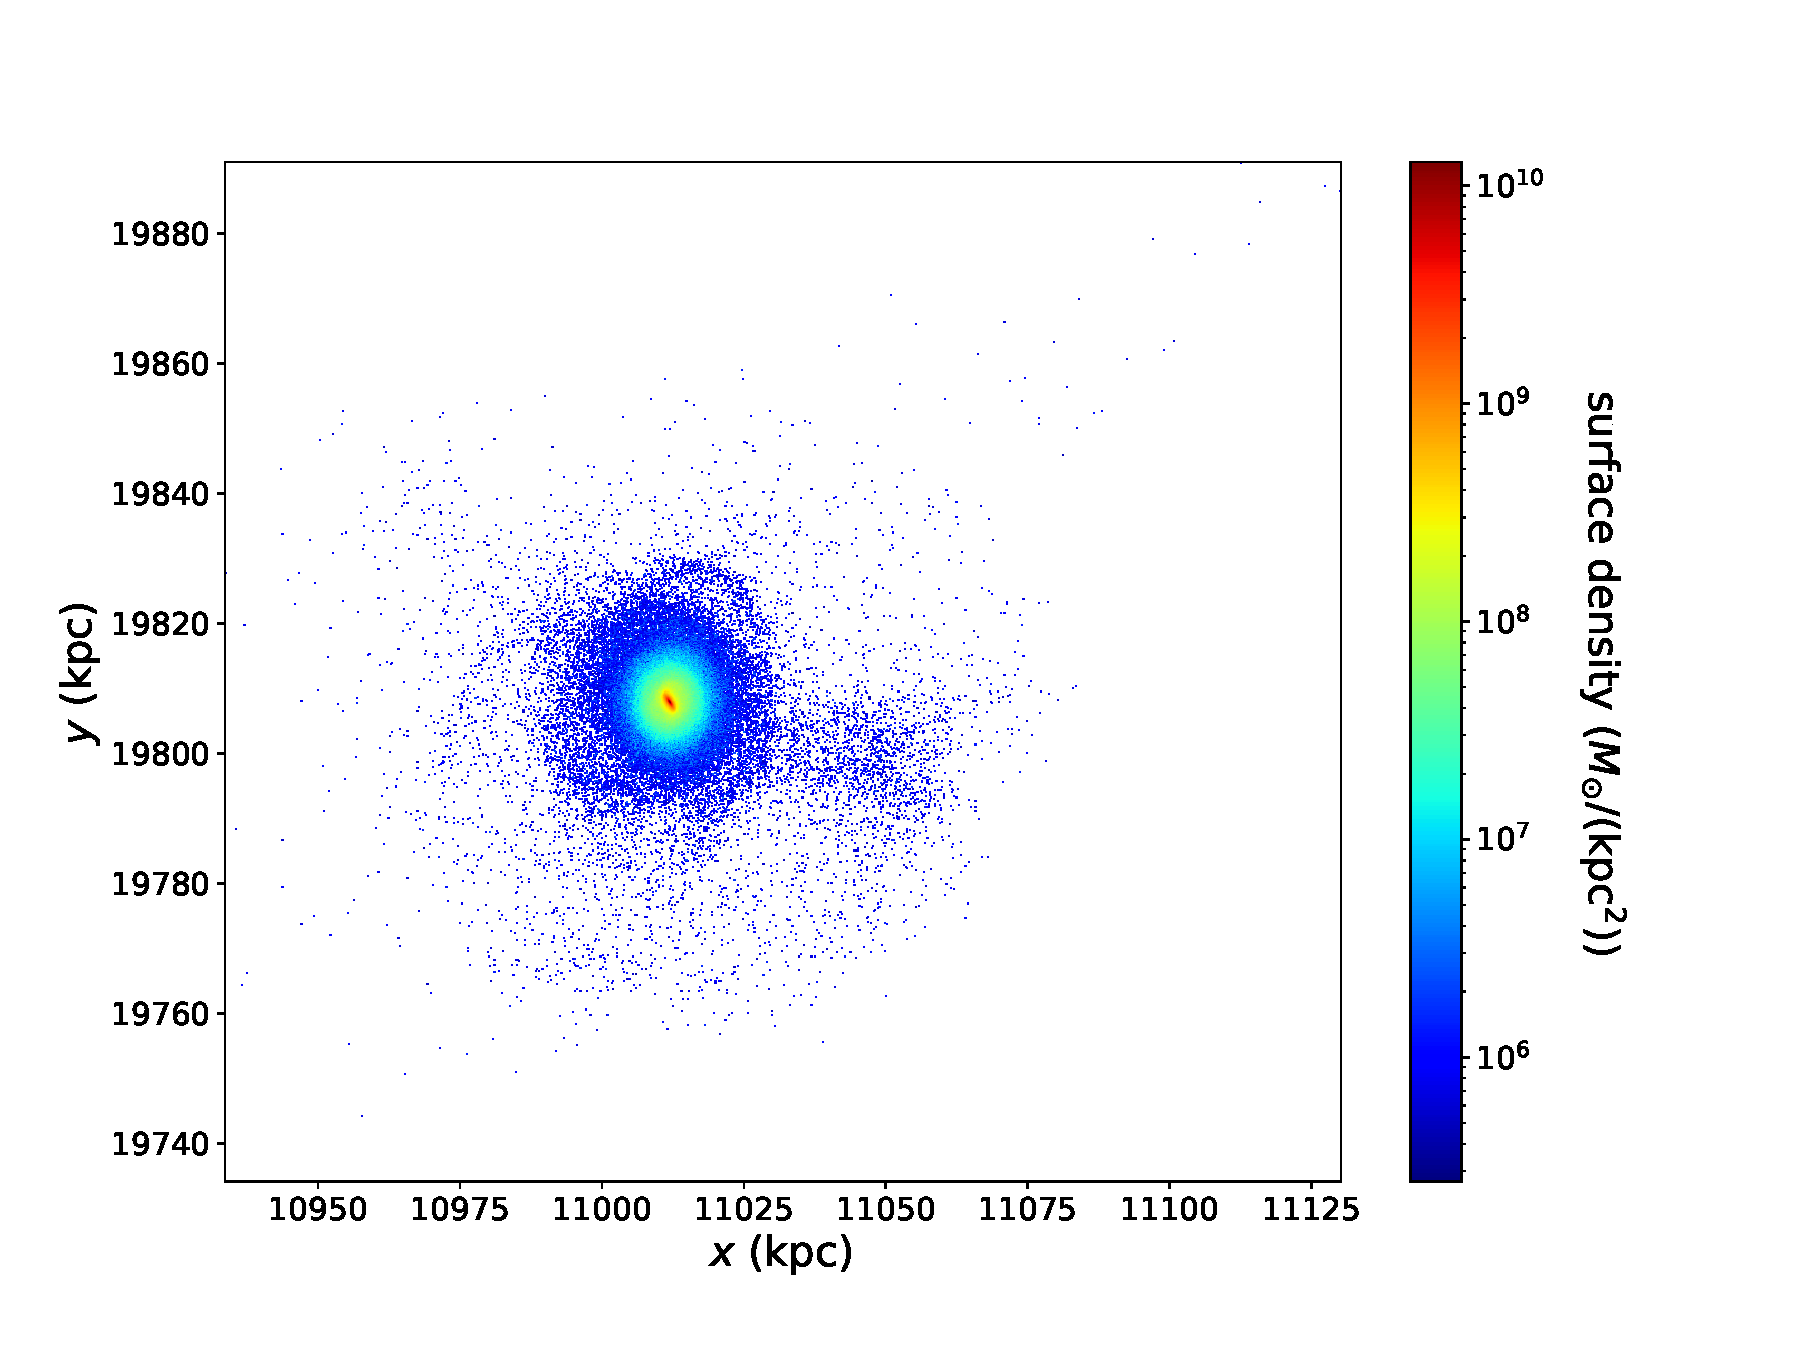
\includegraphics[scale = 0.5]{Figure_1.pdf}
    \caption{Plot of the stellar particles in the reference frame of the simulation box.}
    \label{Fig1}
\end{figure}


\section{Part 2}

In part 2, we want to define a new coordinate system with z-axis is aligned with the direction of the angular momentum of the disk, and plot the surface density in this new system. We first move all the positions and velocities vectors to the reference frame of the center of mass, and calculate the angular momentum using Equation \ref{eq:1}:

\begin{equation} \label{eq:1}
    \Vec{L} = \sum_i m_i \Vec{r}_i \times \Vec{v}_i .
\end{equation}


Then we define a new orthonormal basis $\boldsymbol{e_x}, \boldsymbol{e_y}, \boldsymbol{e_z}$, with $\boldsymbol{e_z}$ aligned with $\Vec{L}$. The old coordinates can be now transformed into the new basis, using a transformation matrix formed by $\boldsymbol{e_x}, \boldsymbol{e_y}$ and $\boldsymbol{e_z}$. The \texttt{numpy} functions such as \texttt{sum()}, \texttt{linalg.norm()}, \texttt{transpose()} and \texttt{linalg.inv()} come in handy in these steps. Figure \ref{Fig2} shows a surface density plot in this new basis.


\begin{figure}[ht]
    \centering
    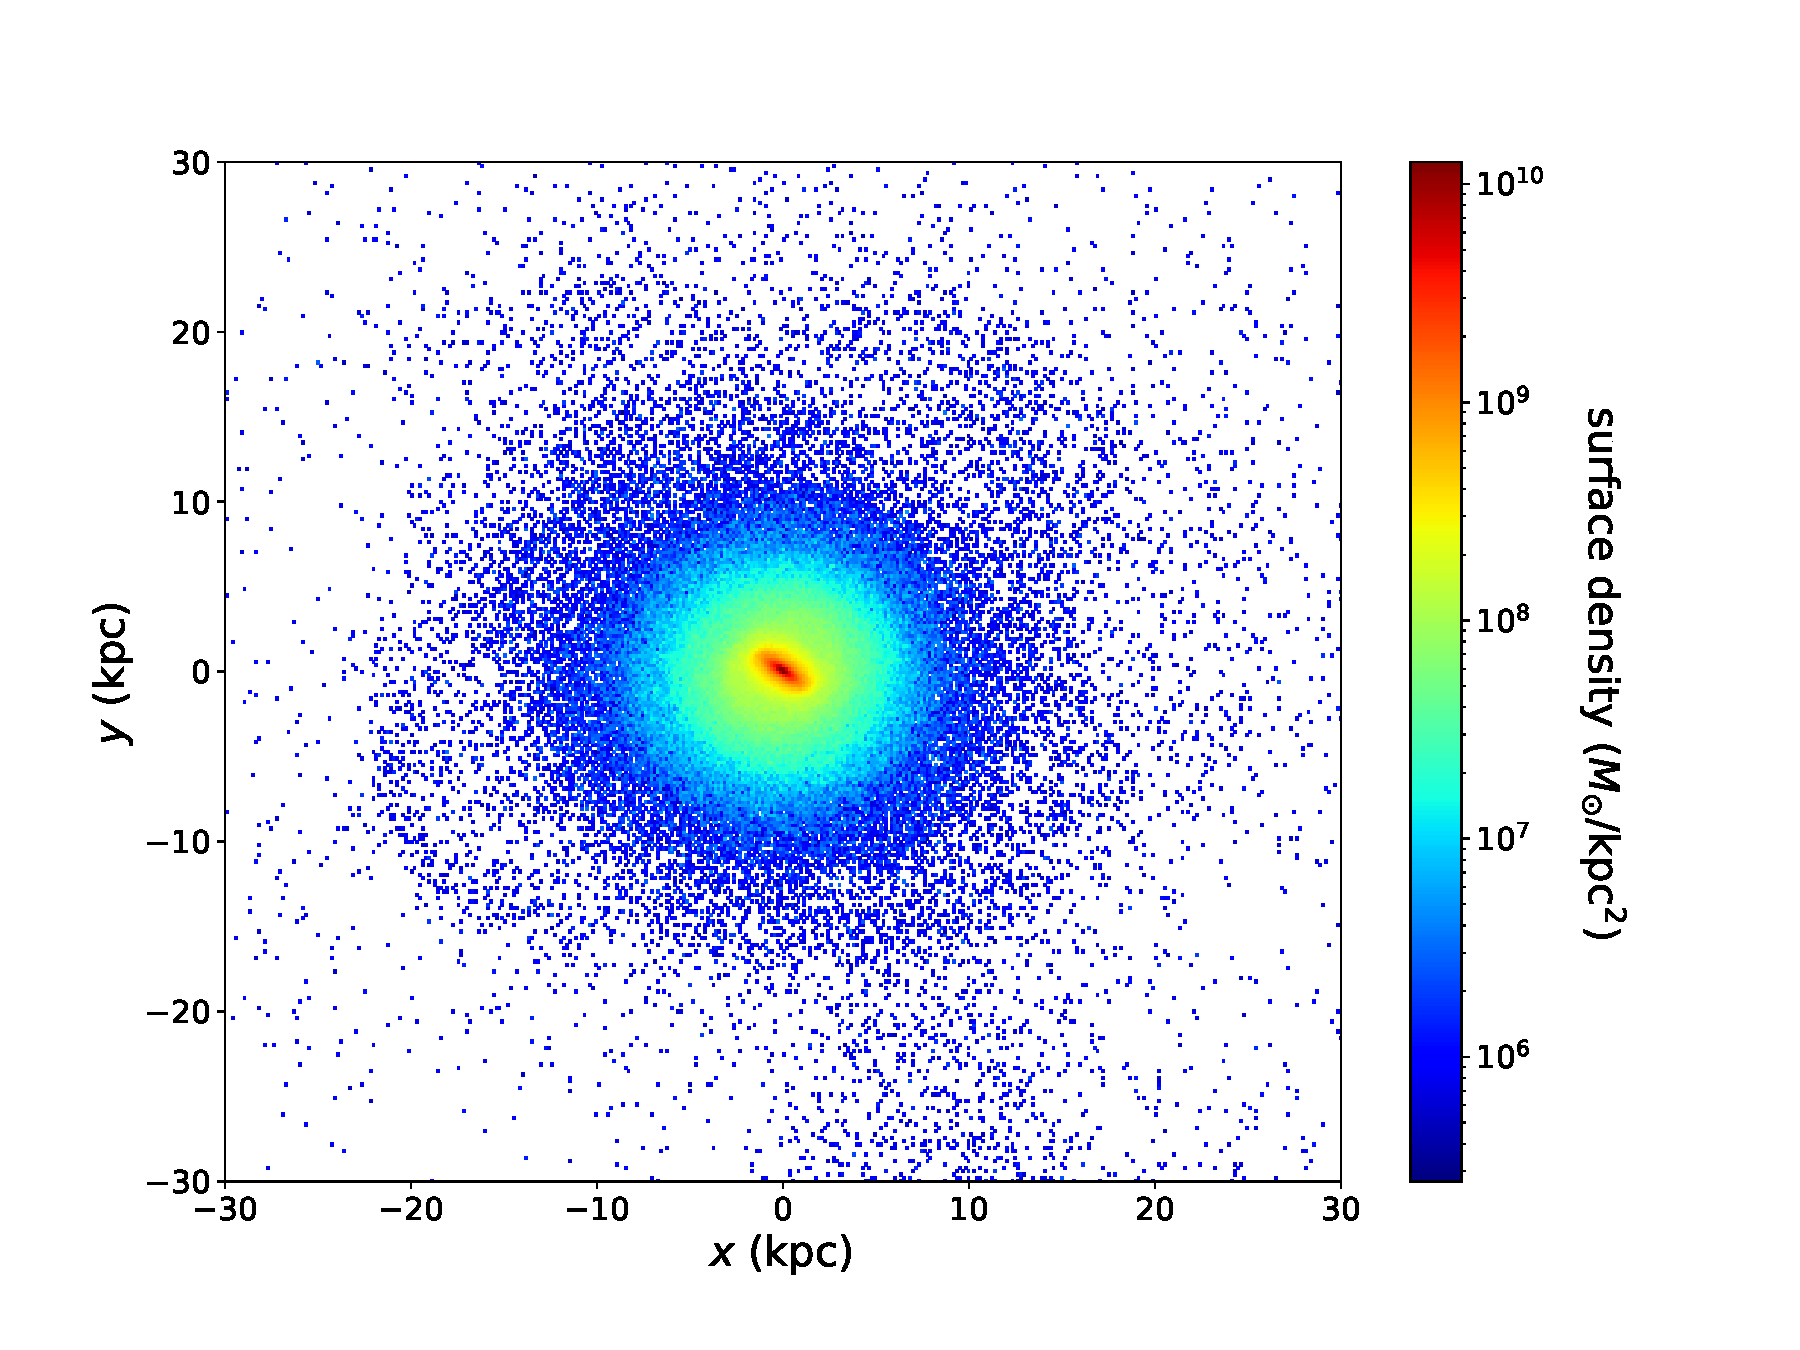
\includegraphics[scale = 0.5]{Figure_2.pdf}
    \caption{Zoomed-in plot of the stellar particles in the new reference frame, where z-axis is aligned with the direction of the angular momentum of the disk.}
    \label{Fig2}
\end{figure}


If we assume that the density profiles $\Sigma$ of disk galaxies are well described by:

$$ \Sigma(R) = \Sigma_0 \exp(-R/R_d),$$

where $R$ is the radius of the disk galaxy. Then:

$$\log \Sigma(R) = \log(\Sigma_0 \exp(-R/R_d)) = \log(\Sigma_0) + \log(\exp(-R/R_d)) = \log(\Sigma_0) + (-R/R_d).$$

Thus if we plot $\log \Sigma$ vs. $R$, the slope of that line would be $k = -\dfrac{1}{R_d}$. The scale-length is then just: $R_d = -\dfrac{1}{k}$. A plot of the log surface density profile is provided in Figure \ref{Fig3}.

\begin{figure}[ht]
    \centering
    \includegraphics[scale = 0.5]{Figure_3.pdf}
    \caption{Plot of the log surface density vs. radial distance from the center, assuming that the the surface density is azimuthally symmetric.}
    \label{Fig3}
\end{figure}

Our calculation based on fit from \texttt{scipy.optimize.curve\_fit} gives the scale-length as about
$R_d =  2.43$ kpc.

\end{document}
